\documentclass[10pt]{article}
\usepackage{mathtools}
\usepackage{pgf-umlcd}
\usepackage{colortbl}
\usepackage{tikz}
\usepackage{verbatim}
\usepackage[left=2cm, right=2cm, top=1cm, bottom=2cm]{geometry}
\title {Computer Science 303: Data Structures Project \#1C\\
\large attachments and source available at https://github.com/alexskc/cs303}
\author{Aleksander Charatonik}
\begin{document}
\maketitle
\begin{section}{Algorithm}
The first step of designing an elevator simulator is to choose an appropriate algorithm, without worrying about implementation, which I will do here. I will start with the most straightforward algorithm that will solve the problem, then consider issues and possible optimizations.\\
\\
The first and most basic solution is to simply take users to the floor they request, in the order the requests come in. The problem with this is immediately apparant. It's not very efficient. If the elevator is already heading up, and a user on the way is also heading up, it makes sense to pick them up along the way, rather than have them "wait their turn."\\
\\
An alternative algorithm that would solve this problem would be to prioritize users going in the in the same up/down direction as the elevator. However, in a single-elevator setup, this is still sub-optimal for a user that is "almost on the way." For example:\\
1. Elevator is on floor 25\\
2. User on floor 1 requests elevator to a floor like 7.\\
3. Elevator starts going down to our user.\\
4. When the elevator is on floor 23, a user arrives on floor 24, requesting floor 1.\\
\\
In this situation, continuing to get the first user would be sub-optimal. The 2nd user would have to wait for the elevator to move 63 floors before they get to where they want. By contrast, if we go back to get the 2nd user, the wait time for the first user only increases by 2.\\
\\
We can fix this by prioritizing users based off how much they are expected to increase wait time, but there is a problem with this: we can get trapped in an infinite loop. For example, if, after the 2nd user showed up and got picked up, we kept adding a new user every 2 turns, the elevator would continue picking them up forever, without getting anyone where they intend to go.\\
\\
In trying to find solutions to this problem, I was not able to find a solution by myself. After doing some research, I found that this is a similar problem to hard disk scheduling. Choosing which direction to send the elavator in is analogous to choosing which direction to send the disk head in. The algorithm I'm looking at is called "Shortest Seek Time First," and the problem of never getting to an old request is called "starvation." What I'm looking to develop is a "starvation-resistant SSTF." Of course, it's easy to design solutions to prevent starvation, such as prioritizing older requests, or some kind of hybrid algorithm. But thes e solutions just aren't very sound.\\
\\
Moreover, SSTF doesn't always necessarily produce the shortest path. For example, if you have a lot of requests on both ends of the elevator, then the algorithm will be drawn to whichever is slightly closer, and then keep moving in that direction and take care of all the requests on one end before taking care of the other half. In these cases, it acts similarly to the standard elevator algorithm. The problem is this: It might've been more efficient to do the other half first. The algorithm has no way of knowing.\\
\\
As we spend more time thinking about this, the problem becomes increasingly apparant: This is a variant of the Travelling Salesman Problem. We can make a few optimizations because an elevator is one-dimensional, but much of the problem still remains... Can we assume that our elevator has infinite computation power? Probably not. We can certainly use a heuristic to make the problem more manageable. With buildings as tall as the Burj Khalifa at a 163 floors, and 63 sectors per track on modern hard drives, we're certainly going to need one. We're certainly not doing 163! or even 63! problems. And one such heuristic is... The elevator algorithm! Back where we started, let's write this one down formally:\\
\\
1. If there are no pending requests, the elevator does nothing.\\
2. As soon as a request is made, the elevator moves toward the requestor. This decides its direction, ascending, or descending.\\
3. If there is a request in the same direction along the way, pick it up as well.\\
4. When there are no requests at the location of the elevator, or further along the direction of the elevator, going in the same direction as the elevator, switch directions.\\
5. Repeat until no requests are left. Stop the elevator until the next request, go back to 1.\\
\\
  \begin{subsection}*{Considerations}
    \begin{itemize}
      \item Users are assumed to know the direction of the elevator. They only enter an elevator going in the same direction they are. In a single-elevator design, the wait time is the same regardless. In a multi-elevator design the wait can be shorter if a 2nd elevator arrives before the first elevator turns around.\\
      \item When an elevator arrives on a floor, all users waiting for it enter, not just one.\\
      \item Behavior can be very different depending on whether the amount of people that can be in an elevator at once is limited or unlimited. While the latter isn't realistic in real-world situations, ideally the software should be able to handle both cases.
      \item For multi-elevator designs, we have to consider which elevator will fullfill the request. This isn't anything more complicated than "the closest elevator that \textit{can} fullfill it. (ie, heading in the same direction or standing still)"
      \item Multiple users should be able to show up and make requests simultaneously.
    \end{itemize}
  \end{subsection}
\end{section}
\begin{section}{Implementation}
  We really only need to keep track of four things:
    \begin{itemize}
      \item The location of each user, either waiting on the floor, or in the elevator. If they get to their destination, we stop keeping track of that user.
      \item The desired location of each user. Desired direction can be inferred by (current location - desired location).
      \item The location of each elevator.
      \item The direction of each elevator.
    \end{itemize}
    Multiple ways of storing these come to mind.
    \begin{itemize}
      \item Store an array of users, and give each user "current location" and "desired location," alongside an array of elevators, each with a "current location" and "direction."
      \item Store an array the size of the number of floors. Each cell represents a floor, and each floor contains an array of users. A second array stores elevators. Each elevator, in turn, stores a direction and an array of users. Users are a single integer, which represents their desired floor.
      \item A combination of the two. For example, using a floor array for users, but giving a location property to elevators.
    \end{itemize}
    I prefer the 3rd method. The 2nd is (subjectively) easiest to visualize, and also means there is no need to traverse the entire array of users if we want to figure out who is above/below the elevator. However, moving elevators becomes expensive if we have to keep copying them from one cell to another to move them. Below is a visualization, followed by a UML diagram:\\
    \begin{tabular}{|>{\columncolor[gray]{0.8}}c | r|}
      \hline
         & Users\\
      \hline
      20 & \\
      \hline
      19 & \\
      \hline
      18 & \\
      \hline
      17 & \begin{tabular}{|c|}
        3
      \end{tabular}\\
      \hline
      16 & \\
      \hline
      15 & \\
      \hline
      14 & \\
      \hline
      13 & \\
      \hline
      12 & \\
      \hline
      11 & \begin{tabular}{| c | c | c | c |}
        15 & 17 & 20 & 7
      \end{tabular}\\
      \hline
      10 & \\
      \hline
      9 & \\
      \hline
      8 & \\
      \hline
      7 & \\
      \hline
      6 & \\
      \hline
      5 & \\
      \hline
      4 & \\
      \hline
      3 & \\
      \hline
      2 & \\
      \hline
      1 & \\
      \hline
      0 & \\
      \hline
    \end{tabular}
\begin{tabular}{|>{\columncolor[gray]{0.8}}c | l|}
      \hline
         & Elevators\\
      \hline
      20 & \begin{tabular}{|>{\columncolor{green}}c | c | c | >{\columncolor{green}}c|}
        \(\downarrow\) & NULL &  & NULL\\
      \end{tabular}\\
      \hline
      19 & \\
      \hline
      18 & \\
      \hline
      17 & \\
      \hline
      16 & \\
      \hline
      15 & \\
      \hline
      14 & \\
      \hline
      13 & \\
      \hline
      12 & \\
      \hline
      11 & \\
      \hline
      10 & \\
      \hline
      9 & \begin{tabular}{|>{\columncolor{green}}c | c | c|}
        \(\uparrow\) & 20 & 20
      \end{tabular}\\
      \hline
      8 & \\
      \hline
      7 & \\
      \hline
      6 & \\
      \hline
      5 & \\
      \hline
      4 & \\
      \hline
      3 & \begin{tabular}{|>{\columncolor{green}}c|}
        NULL
      \end{tabular}\\
      \hline
      2 & \\
      \hline
      1 & \\
      \hline
      0 & \\
      \hline
    \end{tabular}
\\
\\
\\
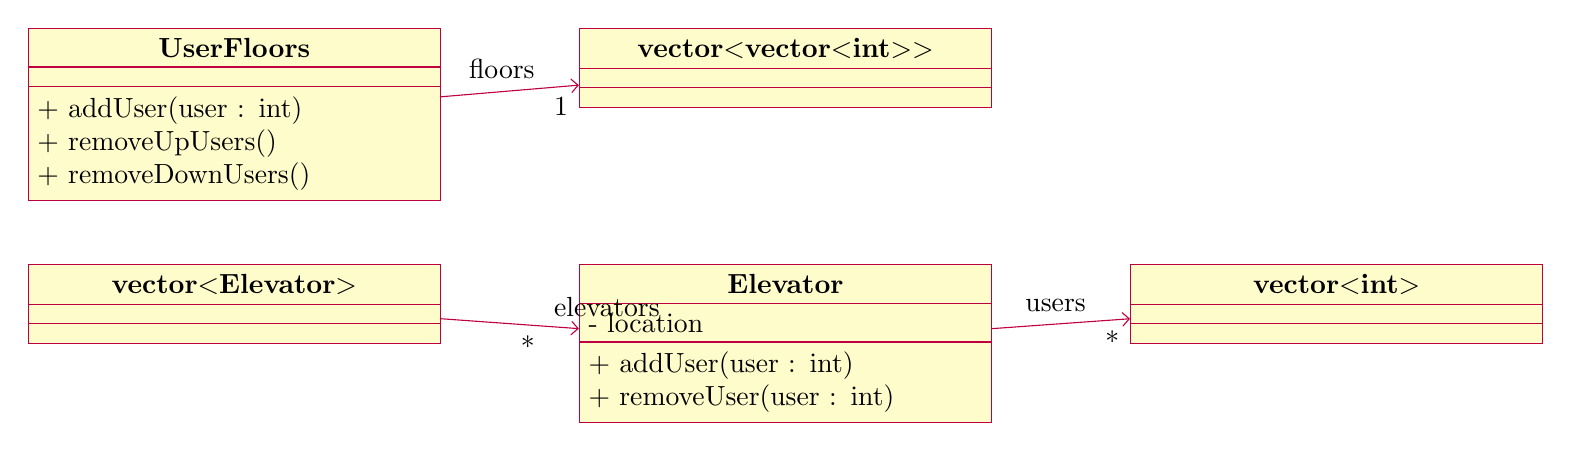
\begin{tikzpicture}
  \begin{class}{UserFloors}{0,0}
    \operation{+ addUser(user : int)}
    \operation{+ removeUpUsers()}
    \operation{+ removeDownUsers()}
  \end{class}
  \begin{class}{vector$<$vector$<$int$>>$}{7,0}
  \end{class}
  \unidirectionalAssociation{UserFloors}{floors}{1}{vector$<$vector$<$int$>>$}

  \begin{class}{vector$<$Elevator$>$}{0,-3}
  \end{class}

  \begin{class}{Elevator}{7, -3}
    \attribute{- location}

    \operation{+ addUser(user : int)}
    \operation{+ removeUser(user : int)}
  \end{class}
  \begin{class}{vector$<$int$>$}{14, -3}
  \end{class}
  \unidirectionalAssociation{vector$<$Elevator$>$}{elevators}{*}{Elevator}
  \unidirectionalAssociation{Elevator}{users}{*}{vector$<$int$>$}
\end{tikzpicture}
\end{section}
\end{document}
